\documentclass{article}

\usepackage{pdfpages}
\usepackage[utf8]{inputenc}
\usepackage{eurosym}
%\usepackage{fancyhdr}
%\pagestyle{fancy}

%
%Die eingegangenen Projektskizzen werden nach folgenden Kriterien bewertet:
%– Zielabdeckung: Das Vorhaben ist auf die Vermittlungsziele des Wissenschaftsjahres 2019 zugeschnitten (Berück-
%sichtigung der Handlungsfelder, Zielgruppen, Forschungsinhalte).
%– Fachliche Kompetenz: Der Antragsteller ist qualifiziert, das Vorhaben durchzuführen und verfügt über nachgewie-
%sene Expertise über das Themenfeld und/oder die Vermittlung des Themenfelds.
%– Schlüssigkeit und Konsistenz des Konzepts: Idee, Ziele, Budgetschätzung.
%– Kommunikative Ausrichtung und Wirksamkeit: Das Vorhaben wird von geeigneten Kommunikationsmaßnahmen be-
%gleitet, es ist öffentlichkeitswirksam und generiert voraussichtlich eine mediale Berichterstattung. Das Vorhaben wird
%kommunikativ in das Wissenschaftsjahr 2018 eingebunden und als Teil dessen wahrgenommen.
%– Innovation: Das Vorhaben ist innovativ und leistet einen Beitrag zur Weiterentwicklung der Wissenschaftskommuni-
%kation in Deutschland.
%– Überregionalität und Nachhaltigkeit: Das Vorhaben strahlt überregional aus und/oder kann übertragen bzw. nachgenutzt werden


\begin{document}


\begin{center}
%\vspace{-13cm}
{ \centering 
\includegraphics[width=10cm]{hsf.png} }

\vspace{-0.8cm}
\begin{figure*}[h!]
\centering
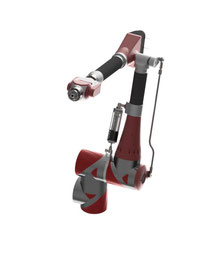
\includegraphics[width=0.6\textwidth]{arm.png}
\end{figure*}
\vspace{-1.8cm}

{\Huge\bf
PROJEKTSKIZZE: Lernen in Handarbeit
}
\\[2em]
\Large
{\bf Antragsteller:} Prof. Dr. Alexander Gepperth (HDR)\\
{\bf Adresse: } Fachbereich Angewandte Informatik der HAW Fulda\\
Leipzigerstr. 123, 36037 Fulda\\
{\bf Email: } alexander.gepperth@cs.hs-fulda.de\\
{\bf Telefon: } 0661 9640 3485\\
\vspace{0.5cm}

{\bf Projektdauer:} 9 Monate\\
\vspace{0.5cm}

{\bf Gesamtkosten:} 150.000\euro\\
\vspace{0.5cm}

{\bf Zuwendungsbedarf:} 150.000\euro\\
\vspace{0.5cm}

%{\bf Konsortium:} Assisted Living, Hilfe für Schwerbehinderte, Service-Robotik, 3D-Simulation
\end{center}
%\end{titlepage}
\newpage

\renewcommand{\thesection}{2}
\section{Antragsteller und assoziierte Partner}
Projektleiter des Projektes ist Herr Prof. Dr. Alexander Gepperth. Prof. Gepperth hat Kompetenzen/Erfahrung/Projekte etc...

\renewcommand{\thesection}{3}
\section{Ausgangsfrage und Ziele des geplanten Vorhabens}

\begin{itemize}
	\item Ziel: Demonstratorsystems zur Visualisierung der Funktionsweise des überwachten Lernens mittels NN
	\item Aufbau eines Handgestenerfassungs + Croppingsystems
	\item Einspeisung + Visualisierung der erfassten Daten für die Benutzer
	\item Visualisierung der Klassifikationsgüte (schlecht - mittel - gut)
	\item Darstellung der Dateneinspeisung, des Trainings, der Veränderung des Netzes + der Verbesserung der Klassifikationsgüte: Lernen durch Beispiele
	\item Deep Dreaming
	\item Handposen vs. Handgesten
	\item Forschungsaspekt: Inkrementelles Lernen

\end{itemize}


\subsection{Kurzzusammenfassung}
\subsection{Grundsätzliche Zielsetzung}
%
\renewcommand{\thesection}{4}
\section{Ausführliche Vorhabensbeschreibung}
gestenerkennung
Dissemination: MINTmachclub, Interaktionsformat, kinderuni,
interaktion mit gymnasialen Oberstufen, interface zur Java oder Python das per Rest die erkannte Geste ausgibt!
webseite
evtl einzelne Leute machen geste, dann halbe Klasse, dann ganze
visualisierung der ausgaben, sicherheit, konfidenz
visualisierung der Prototypen!
visualisierung was gelernt wurde: deep dreaming
ausgabe der berechnungsvotschrift als PDF
message: ist nur ein verfahren, keine Magie
lernen der einschränkungen: linek hand trainieren, rechte testen --> problem!

Die FH Fulda hat tiefgehende Kompetenzen im Bereich des Maschinellen Lernens und modernen Interaktionstechniken. Im Bereich der modernen Interaktionstechniken (insb. Freihandgesten) wurde in bilateralen Forschungsvorhaben ein Demonstrator zur Erkennung von Handgesten mittels 3D-Sensorik entwickelt. Mit Hilfe dieses Demonstrators konnten zahlreiche Erkenntnisse im Bereich des überwachten Lernens, der Sensordatenfusion und der Messung der kognitiven Last im Strassenverkehr gewonnen werden. So wurde in einem kooperativen Forschungsvorhaben nachgewiesen, dass die tatsächliche Ablenkung im Strassenverkehr während der Benutzung von Freihandgesten zur Steuerung von Infotainmentsystemen geringer ist als während der Bedienung durch Touchgesten oder Verwendung analoger Schaltelemente \cite{kopinski2016touch}. 

\begin{figure}[ht]
	\centering
  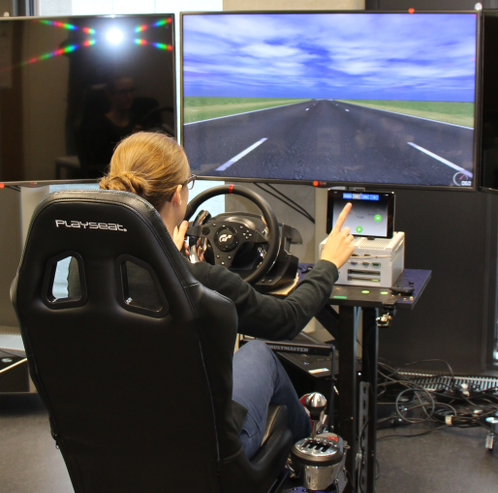
\includegraphics[width=0.7\textwidth]{images/simulator.png}
	\caption{Simulator}
	\label{fig1}
\end{figure}

Hierfür wurde der Demonstrator mit einem Strassenverkehrssimulator gekoppelt und somit konnten realistische Test mittels genormter Messanalysen durchgeführt werden. Aufbauend auf dem Demonstator wurden darüber hinaus zahlreiche Forschungsergebnisse im Bereich der 3D Sensordatenfusion und der mehrstufigen Klassifikation erzielt und veröffentlicht. So waren grundlegende Erkenntnisse, dass Daten aus Time-of-Flight Kameras sowohl früh als auch spät fusionieren um eine Verbesserung der Erkennungsrate zu erzielen \ref{kopinskineural}. Dieses ist insbesondere dahingehend interessant, da es unterschiedliche Performancegewinne des Systems nach sich zieht, was insbesondere für Handgestenerkennung in Echtzeit von hoher Praxisrelevanz ist. Darüber hinaus wurde mit Hilfe von mehrstufigen Neuronalen Netzen nachgewiesen, dass man Informationen aus bereits trainierten Netzen verwenden kann, um eine verbesserte Gesamtperformance des Systems zu erreichen, indem man die Erkennungsgüte mit vortrainierten Netzen stabilisiert \ref{kopinski2015pragmatic}. Diese Erkenntnisse bildeten die Grundlage für die Erkennung von Handposen und die Erkennung von dynamischen Handgesten auf Basis stabiler Posen \ref{kopinski2015real}. Letztlich wurde durch den Einsatz von Deep Learning Verfahren ein eigener Ansatz entwickelt, mittels dessen Erkenntnisse aus dem Bereich der 2D-Bilderkennung in den 3D-Raum übertragen werden konnten \ref{kopinski2016deep}.  

\renewcommand{\thesection}{5}
\section{Darstellung des Eigeninteresses/Eigenanteils}


\renewcommand{\thesection}{6}
\section{Nachhaltigkeit,Übertragbarkeit}
Arbeiten zum inkrementellen Lernen
Arbeiten an Gestenerkennung
Arbeiten an Sequenzerkennung
Einfache Datensammlung
Einsetzbarkeit in der Lehre

\renewcommand{\thesection}{7}
\section{Zeitplan}

\begin{itemize}
\item Projektmanagement Maerz-Dez
\item Aufbau des Systems: Maerz - August
\item Exkursion + Workshop: September - Dezember

\end{itemize}

\renewcommand{\thesection}{8}
\section{Finanzierungsplan}
50\% Stelle Data Science E11 - TVL 11: 27.058,19
50\% Stelle Machine Learning E11 - TVL 11: 27.058,19
Sensoren 1000Euro
Rechner 15000Euro
Depermässigung
2 Hiwis 9 Monate f Visualisierung und Infrastruktur
3 1T SSD-Festplatten für Daten: 2000Euro


\renewcommand{\refname}{}
\bibliographystyle{abbrv}
\bibliography{bib}
%

\end{document}




